\documentclass[12pt]{article}
\usepackage{mathpazo}
\usepackage{tcolorbox}
\usepackage{graphicx}
\usepackage{chngcntr} % allows changing counters
\usepackage{subcaption}  % for subfigures
\usepackage{float}
\usepackage{titlesec}
\usepackage{tabularx}
\usepackage{booktabs}
\usepackage{enumitem}
\usepackage{array}
\usepackage[none]{hyphenat}
\usepackage{ragged2e} 
\usepackage[colorlinks=true, linkcolor=black]{hyperref}
\titlespacing*{\subsubsection}{0pt}{3.25ex plus 1ex minus .2ex}{.7ex}

% Make figure numbers include subsection
\counterwithin{figure}{section}
\counterwithin{table}{section}
% Normal margins
\usepackage[a4paper, margin=1in]{geometry}

% Space between paragraphs
\usepackage{parskip}

% Control line spacing
\usepackage{setspace}
\setstretch{0.95}   % Reduce line spacing slightly

\begin{document}
\pagestyle{empty}
\tableofcontents
\clearpage
\pagestyle{plain}
\setcounter{page}{1} 
\section{Navigation Guide}
\subsection{Menu Structure}
After login, the user lands on the main menu dashboard of the game. At the top of the screen, the user’s profile information is displayed, showing the player name, the current level, and a progress bar indicating the player’s advancement toward the next level.

Below the profile section, the interface presents a vertically arranged menu layout consisting of the following navigation options: \textbf{Your Clan}, \textbf{ClashConnect}, \textbf{Clan Battle}, \textbf{Attack}, and \textbf{Battle History}. These options are displayed as large, clearly separated buttons to allow quick navigation through the main features of the system.

At the bottom of the menu, there is a \textbf{Log Out} button which allows the user to exit the account and return to the login screen. The overall structure provides a simple and organized navigation system for accessing the main functionalities of the application.

\begin{tcolorbox}
\textbf{Note: }The \textbf{Card Interface} at the middle of the screen displays what exactly each button does upon hovering them.
\end{tcolorbox}
\begin{figure}[H]
\centering
\begin{subfigure}{0.38\textwidth}
    \centering
    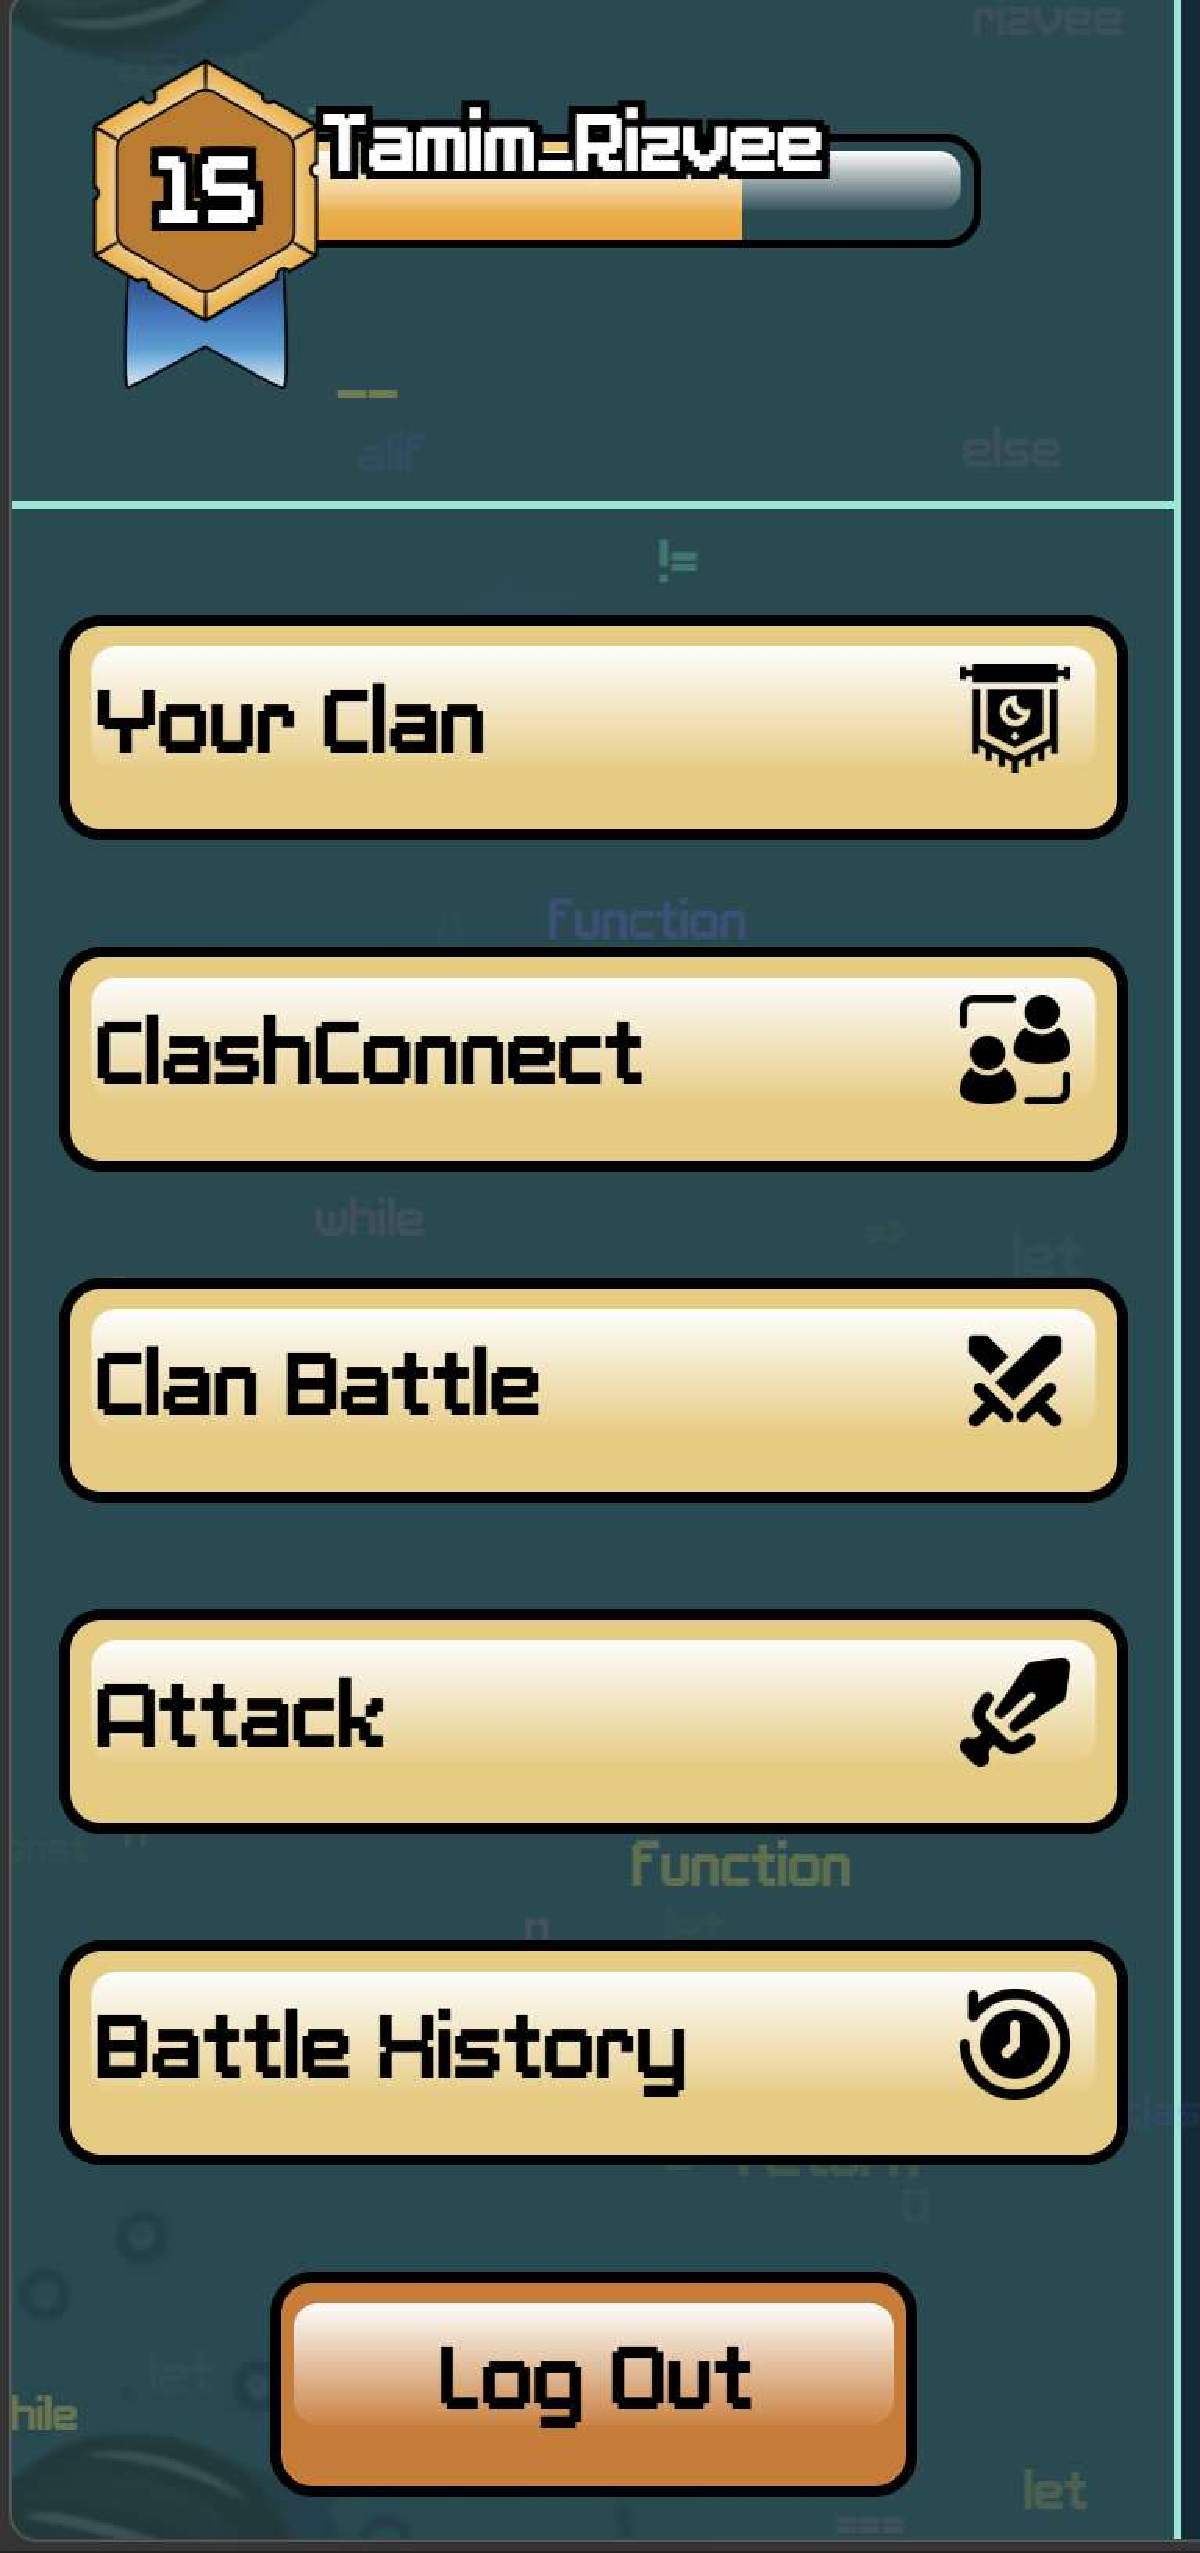
\includegraphics[width=\textwidth]{menu_button.pdf}
    \caption{Main Menu Buttons}
\end{subfigure}
\hfill
\begin{subfigure}{0.38\textwidth}
    \centering
    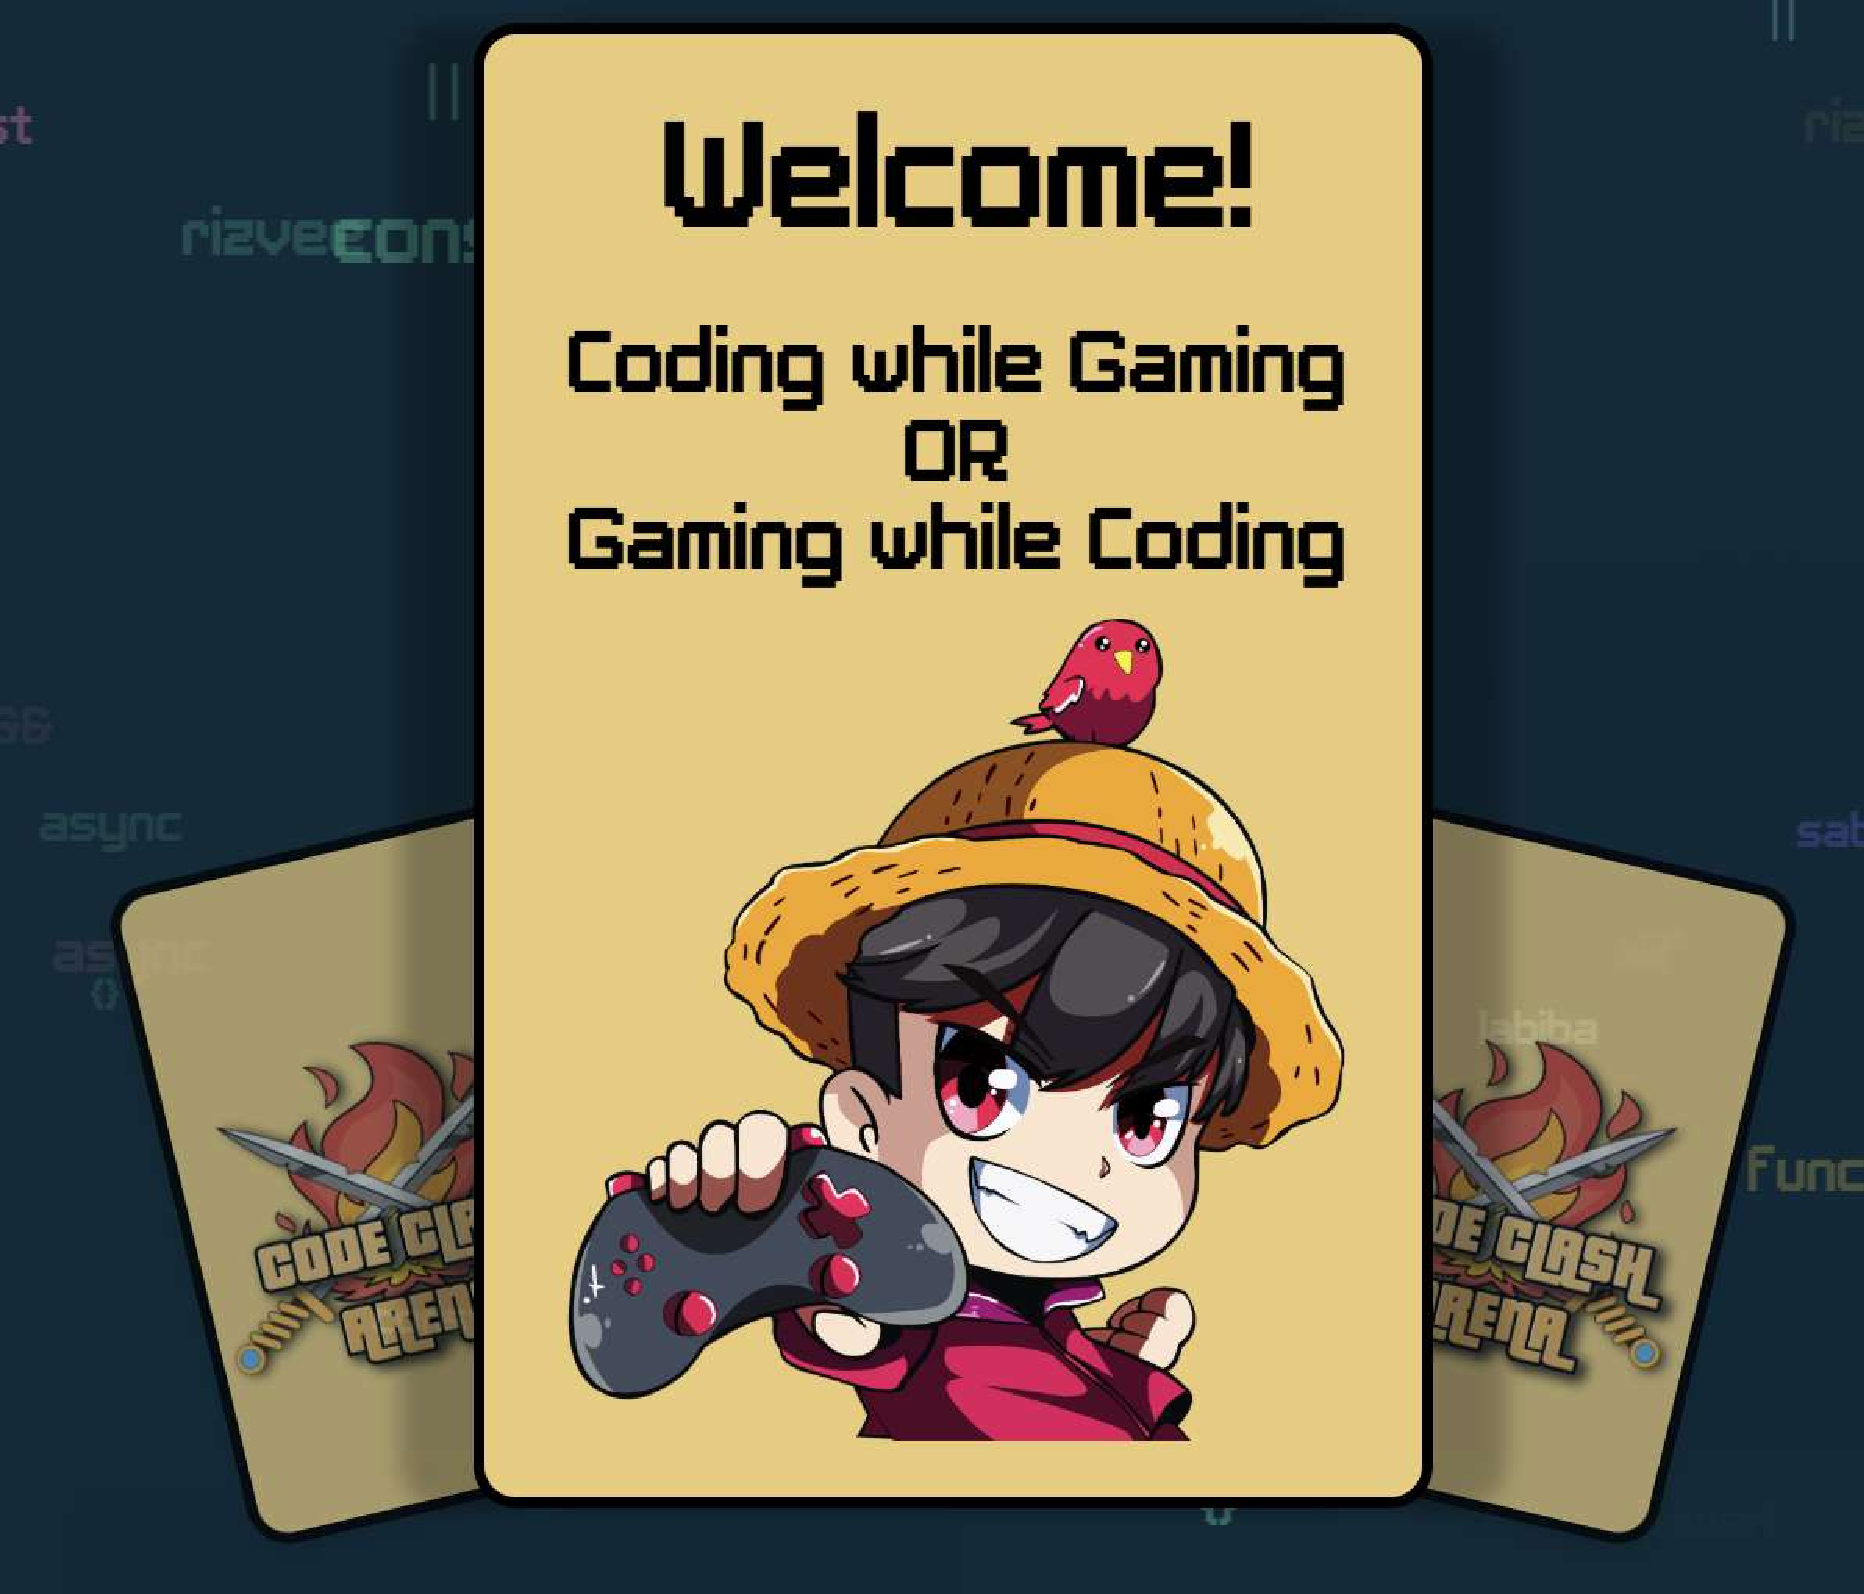
\includegraphics[width=\textwidth]{card.pdf}
    \caption{Card Interface}
\end{subfigure}
\caption{Two Interfaces in Landing Page}
\end{figure}
\subsection{Navigation Options}
\subsubsection{Your Clan}
This button launches a floating menu showing the details of current clan the user belongs and details and ratings of the clan members if the current user is in a clan.Otherwise, the floating menu will show two options for finding a clan or creating a clan.
\subsubsection{Clash Connect}
This button opens a floating menu showing two options. First, it shows a page for finding people and send friend request to them.User can cancel an unaccepted friend request from here. Second, there is a mail page where friend requests sent to user are shown. This menu also shows upcoming clan requests if the user is a leader of a clan.
\subsubsection{Clan Battle}
This button opens a page where user can participate in (if the leader has chosen current user for battle) or spectate ( if the leader has not chosen current user for battle) an ongoing clan battle.
\begin{tcolorbox}
\textbf{Note: }The user must be a member of a clan to avail this feature.
\end{tcolorbox}
\subsubsection{Attack}
Launch the PvP battle menu to compete in 1v1 coding challenges. This button opens an overlay menu with multiple battle mode options: Global Battle Mode (matchmaking with players of similar rating), Local Battle Mode (challenge specific friends), and Practice Gym (solo practice without competition). Select your preferred mode to begin competitive coding.
\begin{tcolorbox}
\textbf{Note: }The user must make some friends to participate in the \textbf{Local Battle Mode}
\end{tcolorbox}
\subsubsection{Battle History}
View your complete battle record and performance statistics. This section displays all your past 1v1 battles and clan battles, showing opponents faced, problems solved, battle
outcomes (win/loss), time taken, and rating changes. Use this feature to analyze your performance trends and track your improvement over time.
\subsubsection{Log Out}
Securely end your current session and return to the homepage. Clicking this button clears your authentication tokens and logs you out of the platform. Always use this option when accessing CodeClash Arena from shared or public computers to protect
your account security.
\newpage
\subsection{Buttons and Icons}
\begin{table}[h]
\centering
\begin{tabularx}{\textwidth}{p{5cm} X}
\toprule
\textbf{Button / Icon} & \textbf{Function} \\
\midrule
\textbf{Close Button} & Closes an overlay menu. \\

\textbf{Leave Button} & Enables user to leave a clan. \\

\textbf{Level Icon} & Clicking on the level copies users' unique ID to the clipboard. \\

\textbf{Accept Button} & Enables user to accept clan or friend requests and local or global battle requests. \\

\textbf{Reject Button} & Enables user to reject clan or friend requests and local or global battle requests. \\

\textbf{Challenge Button} & Enables user to send a 1v1 challenge to a friend. \\

\textbf{Send Request Button} & Enables user to send friend request to an existing user or clan request to an existing clan. \\

\textbf{Cancel Request Button} & Enables user to cancel friend request to an existing user or clan request to an existing clan. \\

\textbf{Enter Button} & Enables user to enter 1v1 battle mode or practice gym. \\

\textbf{Exit Button} & Enables user to exit from 1v1 battle mode or practice gym. \\

\textbf{Submit Button} & Enables user to submit a problem to Codeforces. \\

\textbf{Search Button } & Start the search according  for caln or a existing user.\\

\textbf{View Detail button } & Hovering this button shows friends' details.\\
\bottomrule
\end{tabularx}
\caption{Functions of Different Buttons and Icons}
\end{table}
\newpage
\section{Error Handling and Messages}
\subsection{Authentication Errors}
\begin{table}[h]
\centering
\label{tab:login-errors-revised}

\begin{tabularx}{\textwidth}{>{\raggedright\arraybackslash}p{4cm}
>{\raggedright\arraybackslash}p{5cm}
>{\raggedright\arraybackslash}X}
\toprule
\multicolumn{1}{c}{\textbf{Error Message}} &
\multicolumn{1}{c}{\textbf{Possible Cause}} &
\multicolumn{1}{c}{\textbf{Solutions}} \\
\midrule

\vspace{1pt}``Invalid login credentials'' 
& \vspace{1pt}The entered email or password is incorrect, or formatting issues like extra spaces or wrong capitalization exist.
& \begin{itemize}
\item Check email and password
\item Ensure Caps Lock is off
\item Remove extra spaces
\item Use email instead of Codeforces handle
\item Verify email after signup
\end{itemize} \\ 

\vspace{1pt}``Email not confirmed'' or ``Error fetching user data''
& \vspace{1pt}The account has not been verified via email, preventing successful login.
& \begin{itemize}
\item Check inbox or spam for verification email
\item Click confirmation link
\item Retry login after verification
\end{itemize} \\ 

\vspace{1pt}``Too many login attempts''
& \vspace{1pt}Multiple failed login attempts have temporarily locked the account for security reasons.
& \begin{itemize}
\item Wait 15--30 minutes before retrying
\end{itemize} \\ 

\vspace{1pt}``User already registered'' or ``Email already exists''
& \vspace{1pt}The email is already associated with an existing account.
& \begin{itemize}
\item Use login page
\item Reset password if forgotten
\item Use another email for new account
\end{itemize} \\ 

\vspace{1pt}Field validation error or ``Invalid handle''
& \vspace{1pt}The Codeforces handle provided is incorrect or does not exist.
& \begin{itemize}
\item Verify handle on Codeforces profile page
\item Check spelling and capitalization
\item Create account if needed
\end{itemize} \\
\bottomrule
\end{tabularx}
\caption{Common Login and Authentication Errors}
\end{table}
\newpage
\subsection{Network and Connectivity Errors}
\begin{table}[ht]
\centering
\label{tab:network-errors}

\begin{tabularx}{\textwidth}{>{\raggedright\arraybackslash}p{4cm}
>{\raggedright\arraybackslash}p{5cm}
>{\raggedright\arraybackslash}X}
\toprule
\multicolumn{1}{c}{\textbf{Error Message}} &
\multicolumn{1}{c}{\textbf{Possible Cause}} &
\multicolumn{1}{c}{\textbf{Solutions}} \\
\midrule

\vspace{1pt}``Network error'' or ``Failed to fetch'' 
& \vspace{1pt}The browser or application could not connect to the server due to internet issues, VPN restrictions, firewall blocks, or cached data problems.
& \begin{itemize}
\item Check internet connection
\item Refresh page (F5)
\item Verify firewall settings
\item Disable VPN temporarily
\item Clear browser cache
\item Try a different browser
\end{itemize} \\ \\

\vspace{1pt}``Request timeout'' or ``Connection timeout'' 
& \vspace{1pt}The server did not respond in time, often caused by slow or unstable internet, high bandwidth usage, or network congestion.
& \begin{itemize}
\item Ensure stable connection (5+ Mbps for battles)
\item Close bandwidth-consuming applications
\item Switch to a wired connection
\item Try again after a moment
\end{itemize} \\
\bottomrule
\end{tabularx}
\caption{Common Network and Timeout Errors}
\end{table}

\subsection{Clan Related Errors}
\begin{table}[ht!]
\centering
\label{tab:clan-errors}

\begin{tabularx}{\textwidth}{>{\raggedright\arraybackslash}p{4cm}
>{\raggedright\arraybackslash}p{5cm}
>{\raggedright\arraybackslash}X}
\toprule
\multicolumn{1}{c}{\textbf{Error Message}} &
\multicolumn{1}{c}{\textbf{Possible Cause}} &
\multicolumn{1}{c}{\textbf{Solutions}} \\
\midrule

\vspace{1pt}``Already in a clan'' or ``Join request failed'' 
& \vspace{1pt}The user is currently a member of another clan, or the target clan is not accepting new members or has pending requests. 
& \begin{itemize}
\item Leave current clan before joining another
\item Wait for pending requests to be processed
\item Verify clan is accepting members and you meet requirements
\end{itemize} \\ \\

\vspace{1pt}``Insufficient permissions'' or ``Only clan leader can start battles'' 
& \vspace{1pt}The user does not have the required leadership permissions to initiate a clan battle. 
& \begin{itemize}
\item Contact clan leader to start battle
\item Create your own clan for leadership permissions
\end{itemize} \\
\bottomrule
\end{tabularx}
\caption{Common Clan-related Errors}
\end{table}
\newpage
\subsection{Battle Related Errors}
\begin{table}[h]
\centering
\label{tab:battle-errors}

\begin{tabularx}{\textwidth}{>{\raggedright\arraybackslash}p{4cm}
>{\raggedright\arraybackslash}p{5cm}
>{\raggedright\arraybackslash}X}
\toprule
\multicolumn{1}{c}{\textbf{Error Message}} &
\multicolumn{1}{c}{\textbf{Possible Cause}} &
\multicolumn{1}{c}{\textbf{Solutions}} \\
\midrule

\vspace{1pt}``Connection lost'' or ``Battle disconnected'' 
& \vspace{1pt}The connection between the client and server was interrupted, often due to unstable internet or network congestion. Failure to reconnect may result in automatic forfeit.
& \begin{itemize}
\item Use wired Ethernet connection
\item Ensure stable internet before battles
\item Close unnecessary applications
\item Avoid battles during network instability
\end{itemize} \\ \\

\vspace{1pt}``Submission failed'' or ``Error submitting code'' 
& \vspace{1pt}The code submission could not reach the server or was rejected due to incorrect configuration, network issues, or account problems.
& \begin{itemize}
\item Check internet connection
\item Verify Codeforces handle is correctly linked
\item Ensure Codeforces account is in good standing
\item Retry after a few seconds
\item Verify correct programming language is selected
\end{itemize} \\
\bottomrule
\end{tabularx}
\caption{Common Battle and Submission Errors}
\end{table}
\begin{tcolorbox}
\justifying
\textbf{Note:} Users must not open any screen recorder, snipping tool, or use third-party applications during code submission. Doing so may prevent the submission from being processed, and the problem may not be fetched and displayed. Codeforces has increased its security to ensure fairness and transparency in competitive programming.
\end{tcolorbox}
\end{document}